\documentclass[11pt]{article}
\usepackage{../../latex/stat4ml_style}

\title{Chapter 4: Recommendation Systems \\ \large Part II --- Introduction to Statistical Learning}
\author{Omid Safarzadeh}
\date{}

\begin{document}
\maketitle

\begin{abstract}
\noindent
A recommender is handed a ratings table that is almost entirely blank --- most
users have rated almost no items --- and asked to fill in the gaps. Stated
plainly it is a \emph{matrix completion} problem, and it is hopeless without an
assumption: here, that the full table is approximately \emph{low rank}. That one
assumption turns guessing into estimation. It says every user and every item is
described by a short vector of hidden ``taste'' coordinates, and a rating is
their dot product. This chapter builds that latent-factor model, fits it two
ways --- \keyterm{alternating least squares}, which is nothing but the ridge
regression of Chapter~3 solved one side at a time, and \keyterm{Funk SVD}, which
is stochastic gradient descent over the observed cells --- and shows where the
singular value decomposition sits behind both.
\end{abstract}

\tableofcontents

% ======================================================================
\section{The completion problem and the low-rank assumption}
% ======================================================================

Arrange the data as a matrix $R\in\mathbb{R}^{n\times m}$: $n$ users down the
rows, $m$ items across the columns, and $R_{ui}$ the rating user $u$ gave item
$i$. The defining feature is that only a small set $\Omega$ of entries is
observed --- a few percent is typical --- and the goal is to predict the rest.
With no structure linking the entries this is impossible: the unseen cells are
free parameters, and any completion is as good as any other.

The structural assumption that rescues the problem is that $R$ is, up to noise,
of low \keyterm{rank} $k\ll \min(n,m)$. A rank-$k$ matrix factors as
$R\approx PQ^\top$ with $P\in\mathbb{R}^{n\times k}$ and $Q\in\mathbb{R}^{m\times
k}$, so each user $u$ owns a vector $p_u\in\mathbb{R}^k$, each item $i$ a vector
$q_i\in\mathbb{R}^k$, and the model for a single rating is their inner product.

\begin{definition}[Latent-factor model]
Each user and item is represented by a vector in a shared $k$-dimensional
\keyterm{latent space}, and the predicted rating is
\[
  \hat R_{ui} = p_u^\top q_i = \sum_{f=1}^{k} p_{uf}\,q_{if}.
\]
The $k$ coordinates are not given in advance; they are estimated from the
observed ratings. A coordinate behaves like an unnamed genre: $q_{if}$ is how
much item $i$ expresses factor $f$, and $p_{uf}$ is how much user $u$ cares about
it.
\end{definition}

Low rank is the whole reason the blanks become predictable. A full $n\times m$
table has $nm$ free numbers; the factored model has only $(n+m)k$. When
$k$ is small the handful of observed ratings per user over-determines that
user's $k$ coordinates, and once $p_u$ and every $q_i$ are pinned down, every
missing $R_{ui}$ is simply read off as $p_u^\top q_i$. Sharing the item vectors
$q_i$ across all users is what lets one person's ratings inform another's: this
is why the method is a form of \keyterm{collaborative filtering}.

% ======================================================================
\section{Fitting it: alternating least squares is ridge, twice}
% ======================================================================

We fit $P$ and $Q$ by least squares over the \emph{observed} entries only, with
a ridge penalty to keep the factors from overfitting the few ratings each user
has:
\[
  \mathcal{L}(P,Q)=\sum_{(u,i)\in\Omega}\big(R_{ui}-p_u^\top q_i\big)^2
     +\lambda\sum_u\|p_u\|^2+\lambda\sum_i\|q_i\|^2 .
\]
This objective is not jointly convex in $(P,Q)$ --- the product $p_u^\top q_i$
couples them --- but it is convex in either factor with the other held fixed.
That is the opening for \keyterm{alternating least squares}: freeze $Q$ and
solve for every $p_u$, then freeze $P$ and solve for every $q_i$, and repeat.
Each half-step is an ordinary ridge regression.

\begin{theorem}[The ALS update is the ridge estimator]
Fix the item factors $Q$. Let $\Omega_u=\{i:(u,i)\in\Omega\}$ be the items user
$u$ rated, stack those item vectors as the rows of
$Q_u\in\mathbb{R}^{|\Omega_u|\times k}$ and the ratings as $r_u$. Then the
$p_u$ minimising $\mathcal{L}$ is
\[
  p_u^\star=\big(Q_u^\top Q_u+\lambda I_k\big)^{-1}Q_u^\top r_u,
\]
and the matrix $Q_u^\top Q_u+\lambda I_k$ is invertible for every $\lambda>0$.
\end{theorem}
\begin{proof}
Holding $Q$ fixed, the only terms of $\mathcal{L}$ involving $p_u$ are
\[
  \ell(p_u)=\|r_u-Q_u p_u\|^2+\lambda\|p_u\|^2 .
\]
This is exactly the ridge objective of Chapter~3 with design matrix $Q_u$ and
response $r_u$. Expanding and differentiating,
\[
  \nabla_{p_u}\ell = -2\,Q_u^\top\!\big(r_u-Q_u p_u\big)+2\lambda p_u ,
\]
and setting the gradient to zero gives the normal equations
$\big(Q_u^\top Q_u+\lambda I_k\big)p_u=Q_u^\top r_u$. For invertibility, take any
$v\neq 0$: then
\[
  v^\top\!\big(Q_u^\top Q_u+\lambda I_k\big)v=\|Q_u v\|^2+\lambda\|v\|^2
     \ge \lambda\|v\|^2>0 ,
\]
so the matrix is positive definite and hence invertible. Because $\ell$ is a
strictly convex quadratic (its Hessian $2(Q_u^\top Q_u+\lambda I_k)$ is positive
definite), this stationary point is the unique global minimum.
\end{proof}

The symmetric statement holds for each $q_i$ with $P$ fixed. So one ALS sweep is
$n+m$ independent $k\times k$ ridge solves --- tiny, since $k$ is a handful ---
and each sweep can only lower $\mathcal{L}$, which is bounded below by zero, so
the objective converges. The $\lambda I_k$ term is doing double duty: it is the
Gaussian prior on the factors (Chapter~3's MAP view) \emph{and} the guarantee
that the $k\times k$ system is never singular even when a user rated fewer than
$k$ items.

\begin{lstlisting}[language=Python]
import numpy as np

def als(R, mask, k, lam, sweeps):          # R: n x m, mask: observed entries
    n, m = R.shape
    P = 0.1*np.random.randn(n, k); Q = 0.1*np.random.randn(m, k)
    I = lam*np.eye(k)
    for _ in range(sweeps):
        for u in range(n):                 # each user: one ridge solve
            j = np.where(mask[u])[0]
            Qj = Q[j]
            P[u] = np.linalg.solve(Qj.T@Qj + I, Qj.T@R[u, j])
        for i in range(m):                 # each item: one ridge solve
            v = np.where(mask[:, i])[0]
            Pv = P[v]
            Q[i] = np.linalg.solve(Pv.T@Pv + I, Pv.T@R[v, i])
    return P, Q
\end{lstlisting}

% ======================================================================
\section{Funk SVD: stochastic gradient over the observed cells}
% ======================================================================

ALS solves each factor exactly but needs a $k\times k$ inverse per user and
item. The alternative, popularised during the Netflix Prize as \keyterm{Funk
SVD}, keeps the same objective but walks downhill one observed rating at a time
with stochastic gradient descent (Chapter~3 again). For a single cell $(u,i)$,
write the residual $e_{ui}=R_{ui}-p_u^\top q_i$. The gradient of that cell's
penalised loss is
\[
  \frac{\partial}{\partial p_u}=-2\,e_{ui}\,q_i+2\lambda p_u,\qquad
  \frac{\partial}{\partial q_i}=-2\,e_{ui}\,p_u+2\lambda q_i,
\]
so the SGD step (folding the 2 into the rate $\eta$) nudges each factor toward
the other in proportion to the error:
\[
  p_u\leftarrow p_u+\eta\,(e_{ui}\,q_i-\lambda p_u),\qquad
  q_i\leftarrow q_i+\eta\,(e_{ui}\,p_u-\lambda q_i).
\]
The two factors chase each other: a positive residual pulls $p_u$ along $q_i$
and $q_i$ along $p_u$, raising the next prediction. Real systems add
\keyterm{biases} --- a global mean $\mu$, a user offset $b_u$, an item offset
$b_i$ --- so that $\hat R_{ui}=\mu+b_u+b_i+p_u^\top q_i$, which lets the factors
model \emph{interactions} rather than wasting capacity on the fact that some
users rate high and some items are popular.

\begin{lstlisting}[language=Python]
def sgd_step(p_u, q_i, r, eta, lam):
    e = r - p_u @ q_i                      # residual on this cell
    p_new = p_u + eta*(e*q_i - lam*p_u)    # move p toward q, shrink
    q_new = q_i + eta*(e*p_u - lam*q_i)    # move q toward p, shrink
    return p_new, q_new
\end{lstlisting}

\noindent\textbf{Where the SVD comes in.} The name is a nod to the
\keyterm{singular value decomposition}. If $R$ were \emph{fully observed}, the
Eckart--Young theorem says the best rank-$k$ approximation in squared error is
exactly the truncated SVD, $R\approx U_k\Sigma_k V_k^\top$, which is a
factorisation $PQ^\top$ with $P=U_k\Sigma_k^{1/2}$, $Q=V_k\Sigma_k^{1/2}$. The
recommender problem is the same low-rank fit with two changes the classical SVD
cannot handle: the sum runs over observed entries only, and the ridge penalty
regularises the factors. ALS and Funk SVD are the two standard ways to get the
truncated-SVD idea to work on a matrix full of holes.

\begin{figure}[h]
  \centering
  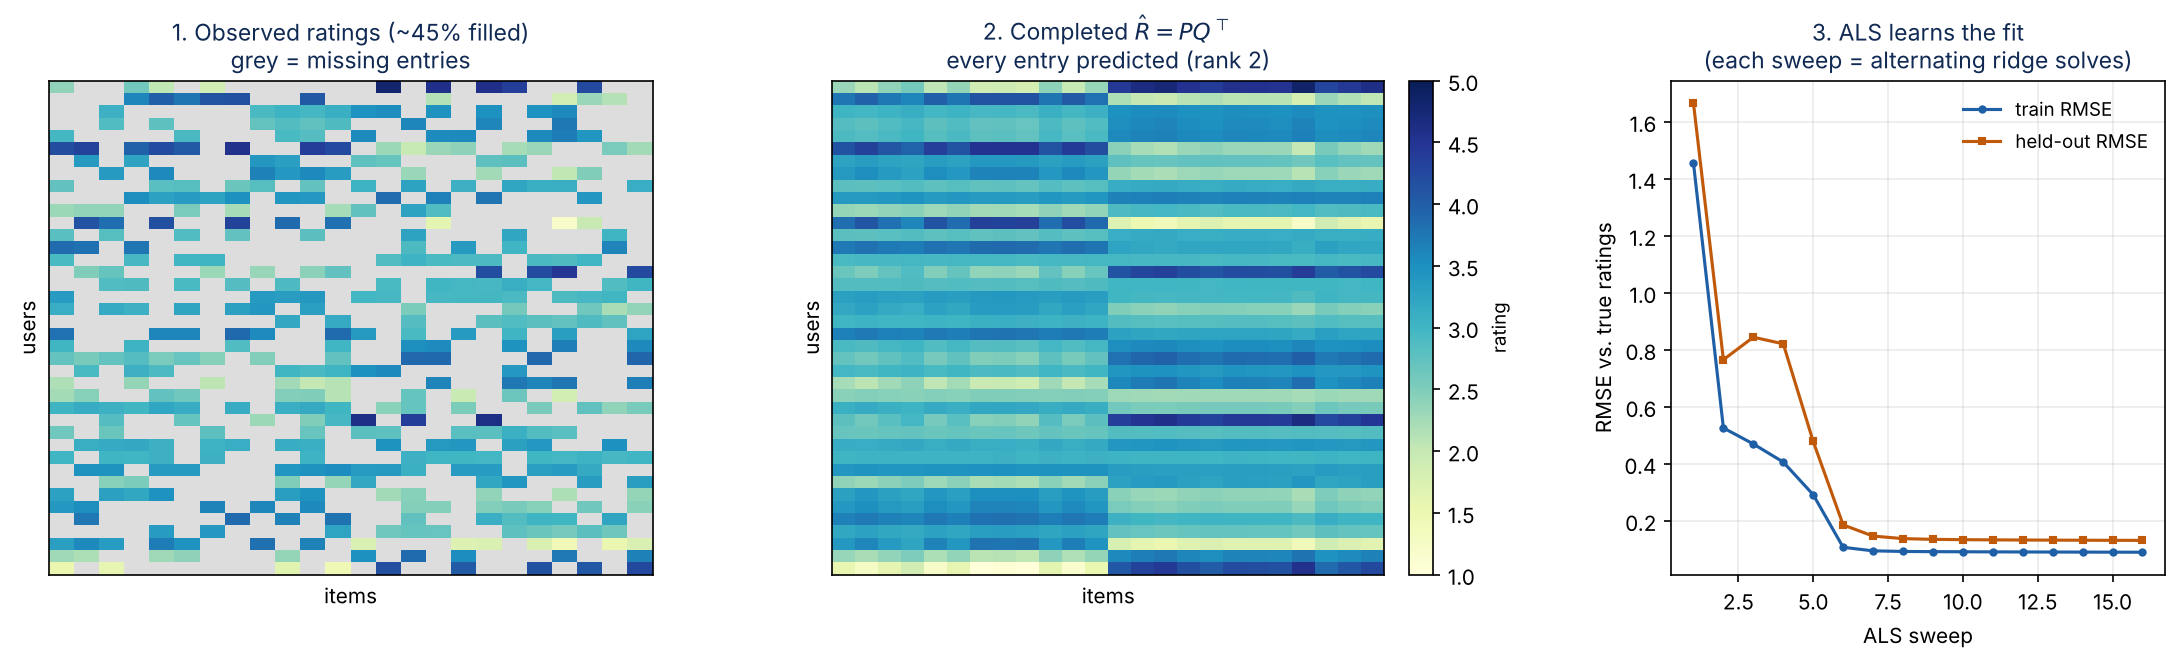
\includegraphics[width=\linewidth]{figures/ch04_panel.png}
\end{figure}

\noindent The figure fits the rank-2 model to a ratings table that is only
$45\%$ observed. The left panel is the raw data, grey where ratings are missing;
the middle panel is the completed $\hat R=PQ^\top$, every cell now predicted ---
and the two latent genres show up as the block structure the factors recovered.
The right panel tracks the error: each ALS sweep is a round of alternating ridge
solves, and both the training and the held-out RMSE fall to the noise floor.

\begin{summarybox}
A recommender is a matrix-completion problem made solvable by the assumption
that the ratings matrix is approximately low rank. The \keyterm{latent-factor
model} gives every user a vector $p_u$ and every item a vector $q_i$ in a shared
$k$-dimensional space and predicts $\hat R_{ui}=p_u^\top q_i$ (plus biases $\mu+
b_u+b_i$ in practice). Fitting minimises the ridge-penalised squared error over
the \emph{observed} entries. \keyterm{Alternating least squares} exploits that,
with one factor fixed, the objective is convex in the other: each update is the
ridge estimator $p_u=(Q_u^\top Q_u+\lambda I)^{-1}Q_u^\top r_u$, provably the
unique minimiser and always well posed for $\lambda>0$. \keyterm{Funk SVD}
optimises the same loss by SGD, stepping each factor toward the other in
proportion to the residual. Both are the truncated SVD (the Eckart--Young
optimum) adapted to missing data and regularisation.
\end{summarybox}

\end{document}
